% Initialisation
\documentclass[english,12pt]{scrartcl}

\usepackage[]{babel}
% Input is utf8
\usepackage[utf8]{inputenc}
% Enables headers and footers
\usepackage[]{scrpage2}
% Lets us colour table cells
\usepackage[table]{xcolor}
% Allows todo list and todos
\usepackage[]{todonotes}
% Makes links in contents hyperlinked
\usepackage{hyperref}
% Make references appear in our table of contents
\usepackage[nottoc,numbib]{tocbibind}
% Allows us to put landscape sections of the document
\usepackage{pdflscape} % \usepackage{lscape} %Use escape for printing (doesn't rotate the pdf page)
% Provides a glossary
\usepackage[toc]{glossaries}

% Gives us pretty diagrams
\usepackage{tikz}
\usetikzlibrary{calc,fit,positioning,chains,decorations.pathreplacing,shapes,backgrounds}

% Document Title and Author
\title{NU-Architecture Requirements Document}
\author{2013 Final Year Project}

% Header and Footer
\pagestyle{scrheadings}
\ihead{\today}
\chead{}
\ohead{NU-Architecture Requirements Document}
\ifoot{}
\cfoot{}
\ofoot{\pagemark}

% Requirements custom commands
\newcommand{\requirement}[1]{\textit{#1}}

% tikz custom shapes
\tikzset{
	old inner xsep/.estore in=\oldinnerxsep,
	old inner ysep/.estore in=\oldinnerysep,
	double circle/.style 2 args={
		circle,
		old inner xsep=\pgfkeysvalueof{/pgf/inner xsep},
		old inner ysep=\pgfkeysvalueof{/pgf/inner ysep},
		/pgf/inner xsep=\oldinnerxsep+#1,
		/pgf/inner ysep=\oldinnerysep+#1,
		alias=sourcenode,
		append after command={
		let \p1 = (sourcenode.center),
		    \p2 = (sourcenode.east),
		    \n1 = {\x2-\x1-#1-0.5*\pgflinewidth}
		in
			node [inner sep=0pt, draw, circle, minimum width=2*\n1,at=(\p1),#2] {}
		}
	},
	double circle/.default={-3pt}{black!80},
	reactor/.style={draw,double circle},
	connection/.style={
		->,
		line width=0.2em
	},
	write/.style={
		->,
		thick
	},
	read/.style={
		<-,
		thick
	},
	readwrite/.style={
		<->,
		thick
	}
}

% Skip line rather then indent paragraphs
\setlength{\parindent}{0.0in}
\setlength{\parskip}{0.1in}

% Make our glossary
\makeglossaries

% Our glossary
\newglossaryentry{powerplant}
{
	name=Power Plant,
	description={
		is the central component of the Proposed Architecture that links all other components together
	}
}

\newglossaryentry{reactor}
{
	name=Reactor,
	description={
		is the reactor
	}
}

\newglossaryentry{reaction}
{
	name=Reaction,
	description={
		is the reaction
	}
}

\newglossaryentry{nubots}
{
	name=NUBots,
	description={
		is the NUBots
	}
}

\newglossaryentry{robocup}
{
	name=RoboCup,
	description={
		is the robocup
	}
}

% Start of document
\begin{document}
	\maketitle
	\vfill
	{\large
		\begin{description}
			\item [Status:] Draft
			\item [Version:] 0.9
		\end{description}}

	\clearpage
	\listoftodos
	\tableofcontents
	\clearpage

	\section{Document Notes}
		\begin{tabular}{ p{0.1\textwidth} | p{0.6\textwidth} | p{0.3\textwidth} }
			\textbf{Version} & \textbf{Changes} & \textbf{Author} \\
			\hline

			0.1 &
			Initial Template &
			Jake Woods \\
			\hline

			0.2 &
			Non-Goals, Requirements (Multithreading, Portability, Performance, Consistent
			Interfaces, New Components), Extension Goals (ROS Support) &
			Jake Woods \\
			\hline

			0.3 &
			Initial Latex Version, Requirements (Networking, Debugging, Unit Testing) &
			Trent Houliston \\
			\hline

			0.4 &
			Current and Proposed System Diagrams, Placeholders for sections &
			Trent Houliston, Jake Woods \\
			\hline

			0.5 &
			Updated Requirements Diagrams and Descriptions (Current and Proposed) &
			Jake Woods \\
			\hline

			0.6 &
			Updates and added more diagrams and massively extended the overview. &
			Jake Woods \\
			\hline

			0.7 &
			Started work on Threading Diagram, cleaned up the latex source and fixed spelling &
			Trent Houliston \\
			\hline

			0.8 &
			Finished Threading Diagram, added bibtex references, extended existing architecture
			overview &
			Trent Houliston, Jake Woods \\
			\hline
			
			0.9 &
			Added Scenario Descriptions and Examples. Large overview changes &
			Trent Houliston, Jake Woods \\
			\hline
		\end{tabular}
		
	\section{Introduction}
		Sometimes in software it is important to take a step back and evaluate your creation.
		The University of Newcastle \gls{nubots} team have in previous years achieved success in the \gls{robocup} competition, placing several times.
		However in recent years the team has undergone a change in robotic platform from the \emph{Aldebaran Nao} to the \emph{Robotis DARwIn-OP}, as well as making continuous compromises in code quality to achieve deadlines.
		As a result of this, the software architecture of the current system has become a bastardised version of its original intent.
		The \gls{nubots} team, as a result of this have decided to replace the existing architecture with a new more effective architecture.
		
		This document outlines the existing architecture, what benefits can be gained from its replacement as well as the issues that warrant its replacement.
		Additionally we also propose a new architecture designed to address these issues as well as providing enhancements that will allow the system to perform effectively now and into the future.
		
		Finally this document outlines the criteria by which this proposed architecture will be measured. 
		We achieve this by providing a list of requirements that the proposed architecture must satisfy.

	\section{Overview}
		This section provides an overview of the existing architecture and the proposed architecture.

		\subsection{Existing Architecture}

			\todo[inline]{Provide a high level overview of the old system and the way it works}

			\begin{figure}
				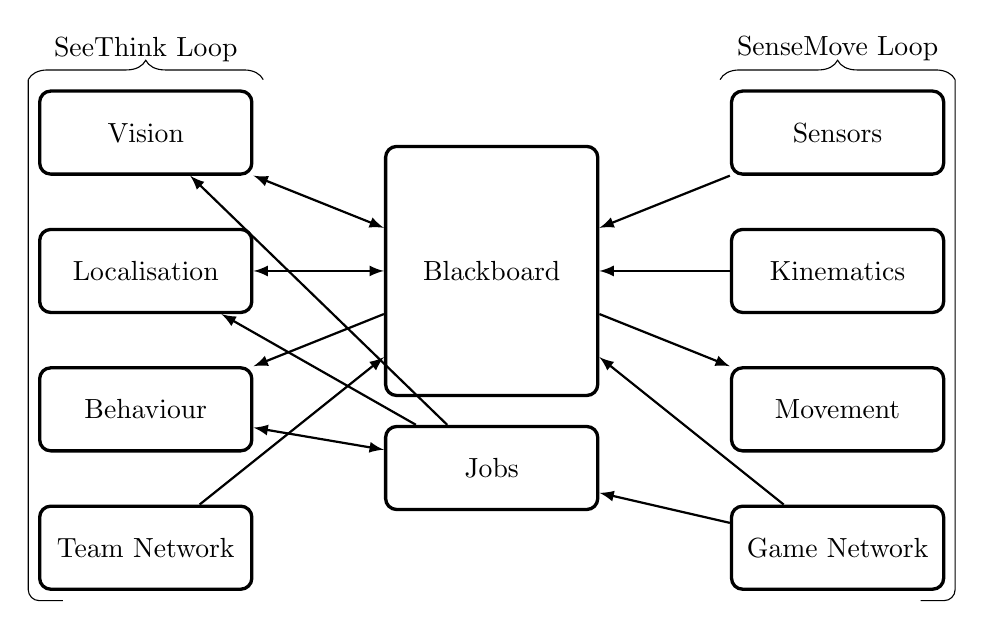
\begin{tikzpicture}[
					x=12.5em,y=5em,
					component/.style={
						rectangle,
						rounded corners,
						draw=black, very thick,
						text width=7em,
						minimum height=3em,
						text centered
					},
					>=latex]

					%%% Nodes
					%% Left hand Side
					\node at (0,3) [component] (vision) {Vision};
					\node at (0,2) [component] (localisation) {Localisation};
					\node at (0,1) [component] (behaviour) {Behaviour};
					\node at (0,0) [component] (teamnetwork) {Team Network};

					%% Center
					\node at (1, 2) [component,minimum height=9em] (blackboard) {Blackboard};
					\node [below=1em of blackboard,component] (jobs) {Jobs};

					%% Right hand side
					\node at(2,3) [component] (sensors) {Sensors};
					\node at(2,2) [component] (kinematics) {Kinematics};
					\node at(2,1) [component] (movement) {Movement};
					\node at(2,0) [component] (gamenetwork) {Game Network};

					%%% Connections
					%% Left hand blackboard connections
					\path [readwrite] (vision) edge (blackboard);
					\path [readwrite] (localisation) edge (blackboard);
					\path [read] (behaviour) edge (blackboard);
					\path [write] (teamnetwork) edge (blackboard);

					%% Left hand jobs connections
					\path [read] (vision) edge (jobs);
					\path [read] (localisation) edge (jobs);
					\path [readwrite] (behaviour) edge (jobs);

					%% Right hand blackboard connections
					\path [write] (sensors) edge (blackboard);
					\path [write] (kinematics) edge (blackboard);
					\path [read] (movement) edge (blackboard);
					\path [write] (gamenetwork) edge (blackboard);

					%% Right hand jobs connections
					\path [write] (gamenetwork) edge (jobs);

					%%% Decorations
					%% SeeThink header
					\node[fit=(vision)(localisation)(behaviour)(teamnetwork)](leftgroup){};
					\draw[rounded corners]
						(leftgroup.north west)--(leftgroup.south west) -- ++(0.10,0);
					\draw[decorate,decoration={amplitude=7pt,brace}] % Header line
						(leftgroup.north west) -- (leftgroup.north east);

					\node[above=1.1em of leftgroup,anchor=center]{SeeThink Loop};

					%% SenseMove header
					\node[fit=(sensors)(kinematics)(movement)(gamenetwork)](rightgroup){};
					\draw[rounded corners]
						(rightgroup.north east) -- (rightgroup.south east) -- ++(-0.10,0);
					\draw[decorate,decoration={amplitude=7pt,brace}]
						(rightgroup.north west) -- (rightgroup.north east);
					\node[above=1.1em of rightgroup,anchor=center]{SenseMove Loop};
				\end{tikzpicture}
				\caption {The existing architecture}
				\label {fig:HighLevelExistingArchitecture}
			\end{figure}

			From a distance, the existing architecture's connections resemble an intricate spider web
			woven from good intentions and demonic pacts with the compiler.
			A highly simplified diagram of the architecture and flow of the existing system can be seen in Figure~\ref{fig:HighLevelExistingArchitecture} on page~\pageref{fig:HighLevelExistingArchitecture}.
			The current system was originally designed as a purely object-oriented system designed to be easy to understand and extend.
			However, the time, deadlines and a lack of understanding of the system have taken their toll. 
			Years of having no one responsible for the architecture has resulted in it slowly fragmenting and has heavily impacted its quality.
			New engineers working on the system had no one to turn to for advice and resorted to implementing unique architectures for their components.
			These problems result in a system with components that use very different assumptions and design patterns.
			This causes duplication of effort for the \gls{nubots} team and it is not uncommon to see very similar classes be implemented multiple times by different people due to the lack of clear architecture.

			Some components communicate through the a global data store known as the blackboard, others utilise a global queue known as the jobs system, most communicate through direct function calls and some components even communicate through implicit or global state such as singletons.
			This myriad of ways in which components can communicate has a huge impact on team productivity.
			In order to make modifications to a component you must understand its interface, the interface of anything it interacts with, and the interfaces of any new component to be used.
			In the \gls{nubots} case it is common to have components that need to talk to three or more other components. This results in a minimum of four different systems you need to understand before you can make any change.

			For example: The vision system communicates utilising a two step process.
			First the vision system accesses the sensor system directly through blackboard and asks it to process a new frame.
			It then waits on the sensor system to place the frame information on blackboard.
			Once the frame information is placed on blackboard the vision system then reads the information
			from blackboard and continues its processing.
			While the vision system is waiting for a new frame the entire robot is blocked and cannot make any decisions.
			It is also important to note that no other systems are intended to request the latest frame, and doing so would break the robots functionality.

			Another example of these architectural issues can be found in the Movement module:
			The \gls{nubots} system defines a number of movement handlers each responsible for a set of movements such as kicking the ball or walking.
			The movement system periodically retrieves all of the jobs in the job queue and sends them to the appropriate movement handler. 
			The movement handlers then talk to the action system to execute the selected motions. 
			This base case does not have any issues however it is also possible for any other component to talk to the movement handlers directly.
			Therefore, at any point in time any class in the system is a potential candidate for triggering a movement making it very difficult to track down which class is responsible for an action, further adding to the complexity of the system.

			The architecture of this section is worse considering that each movement handler is indirectly dependant on the others.
			Movement handlers can lock specific motors and if they attempt to use a motor in use by another system, the action will fail.
			Forgetting to check if you have ownership of a motor can break the currently executing motion causing the robot to fall down and possibly injure itself.

			Thus, in order to add a new movement not only do you need to write the code for the movement
			but you also need to understand how NUMotion, NUWalk, NUKick, NUHead work and interact.
			You need to understand all the cases where any of the managers might be triggered to avoid interrupting a critical movement when the motors are locked.
			You need to understand the locking model to prevent accidentally trying to move a motor you shouldn't.
			These two examples are only two of the pitfalls that await you in the existing architecture.

			\todo[inline] {Expand the description of the Current Architecture}
			
		\subsection{Proposed Architecture}
			\begin{figure}[h]
				\centering
				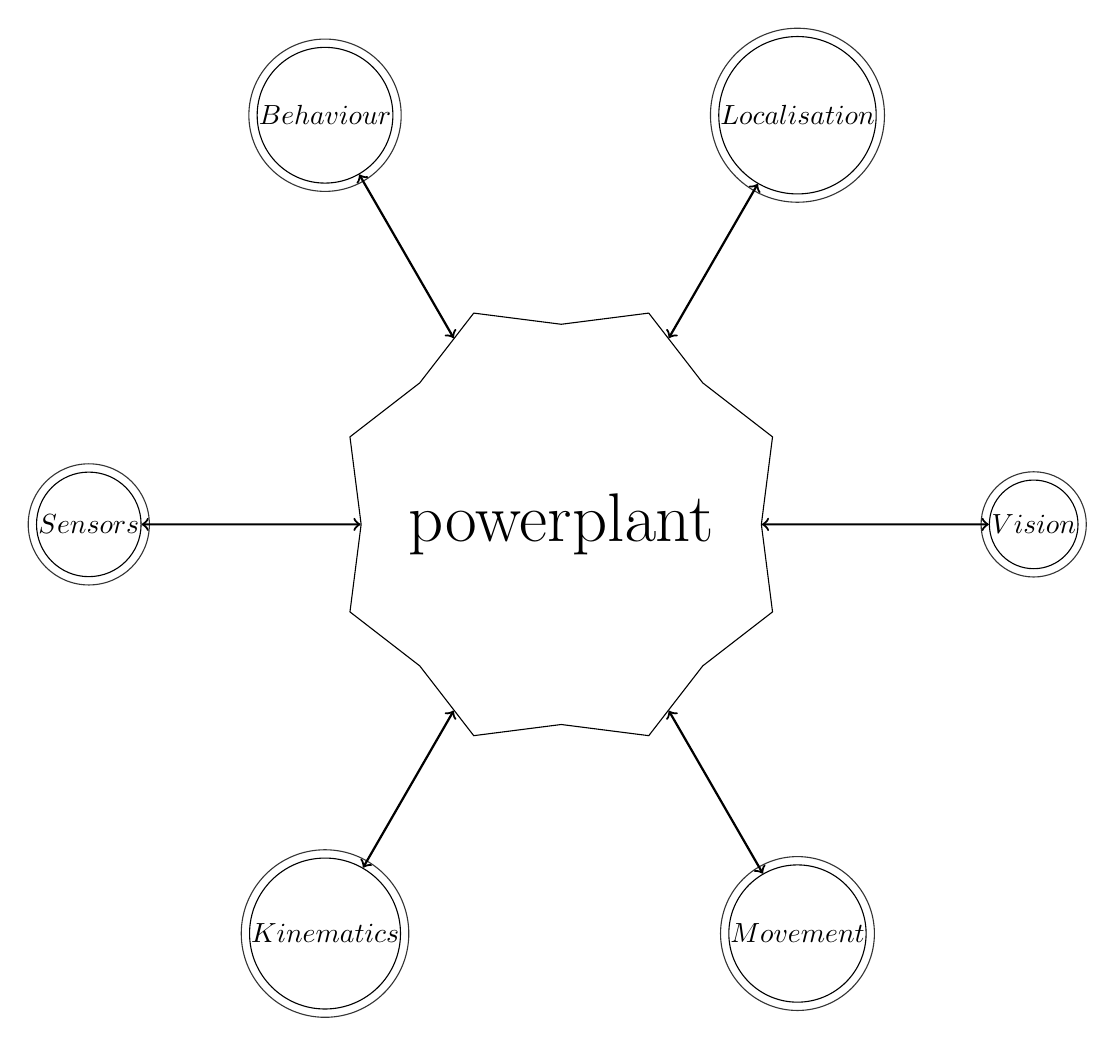
\begin{tikzpicture}

					% Draw our central Power Plant star
					\node [draw,star,star points=8,star point ratio=0.875,minimum width=5cm]
					(powerplant) {\Huge \gls{powerplant}};

					% Loop through each of our reactors
					\foreach [count=\i] \reactor in
					{Vision,Localisation,Behaviour,Sensors,Kinematics,Movement} {

						% Draw the reactors around the central star
						\node[draw,reactor] (reactorcircle) at ({360/6 * (\i - 1)}:6cm)
						{$\reactor$};

						% Draw a line from our reactor to our powerplant
						\path[readwrite] (reactorcircle) edge (powerplant);
					};
				\end{tikzpicture}
				\caption {The proposed architecture}
				\label{fig:HighLevelProposedArchitecture}
			\end{figure}

			The central authority of the proposed architecture is known as the \gls{powerplant} (Figure~\ref{fig:HighLevelProposedArchitecture} page~\pageref{fig:HighLevelProposedArchitecture}).
			The \gls{powerplant} is responsible for the primary communication functions of the architecture through a publish/subscribe message passing system.
			Only one \gls{powerplant} exists can per program and the majority of the time developers of the system will not directly interact with it.

			The primary point of interaction for most users will be a \emph{\gls{reactor}}.
			When a user wants to create a new feature they create a new class that inherits from gls{reactor}.
			This gives them access to the key functionality of the proposed architecture. This functionality revolves around two functions, \textbf{On} and \textbf{Emit}.
			
			\emph{On} allows users to specify \glspl{reaction} which behave as callbacks that are activated when new data comes in. This is the method that is used to obtain data in a loosely coupled manner. The On method does not discriminate which component the data came from. This will be used by the robot in order to build on the results of previous components and perform logic.
			
			There are also a number of special types provided by the system.
			These types can be used in an \emph{On} statement in order to get different behaviour.
			The best example of this is the Every type. This type when used will make the system trigger the On method at regular intervals.
			This functionality will be used by the NUBots as the primal events that trigger all of the sensor reads each round.
			
			\emph{Emit} allows \glspl{reactor} to push data into the \gls{powerplant} that will then distributed to all components that are interested in this datatype. This is done by calling their appropriate \emph{On} methods while providing the Emitted data as a paramter.
			This will be used by the robot to push the results of any operations it has performed to allow other components to use them.
			
			An example: A Sensors reactor reads a camera frame every 30ms and uses \emph{Emit} to push a camera frame to the Power Plant. This is then received by the Vision system that processes the image and outputs the processed image it has created. This sequence of events is shown in Figure~\ref{fig:OnAndEmitExample} on page~\pageref{fig:OnAndEmitExample}.
			
			% On Emit and Every flow diagram
			\begin{figure}[b]
				\centering
				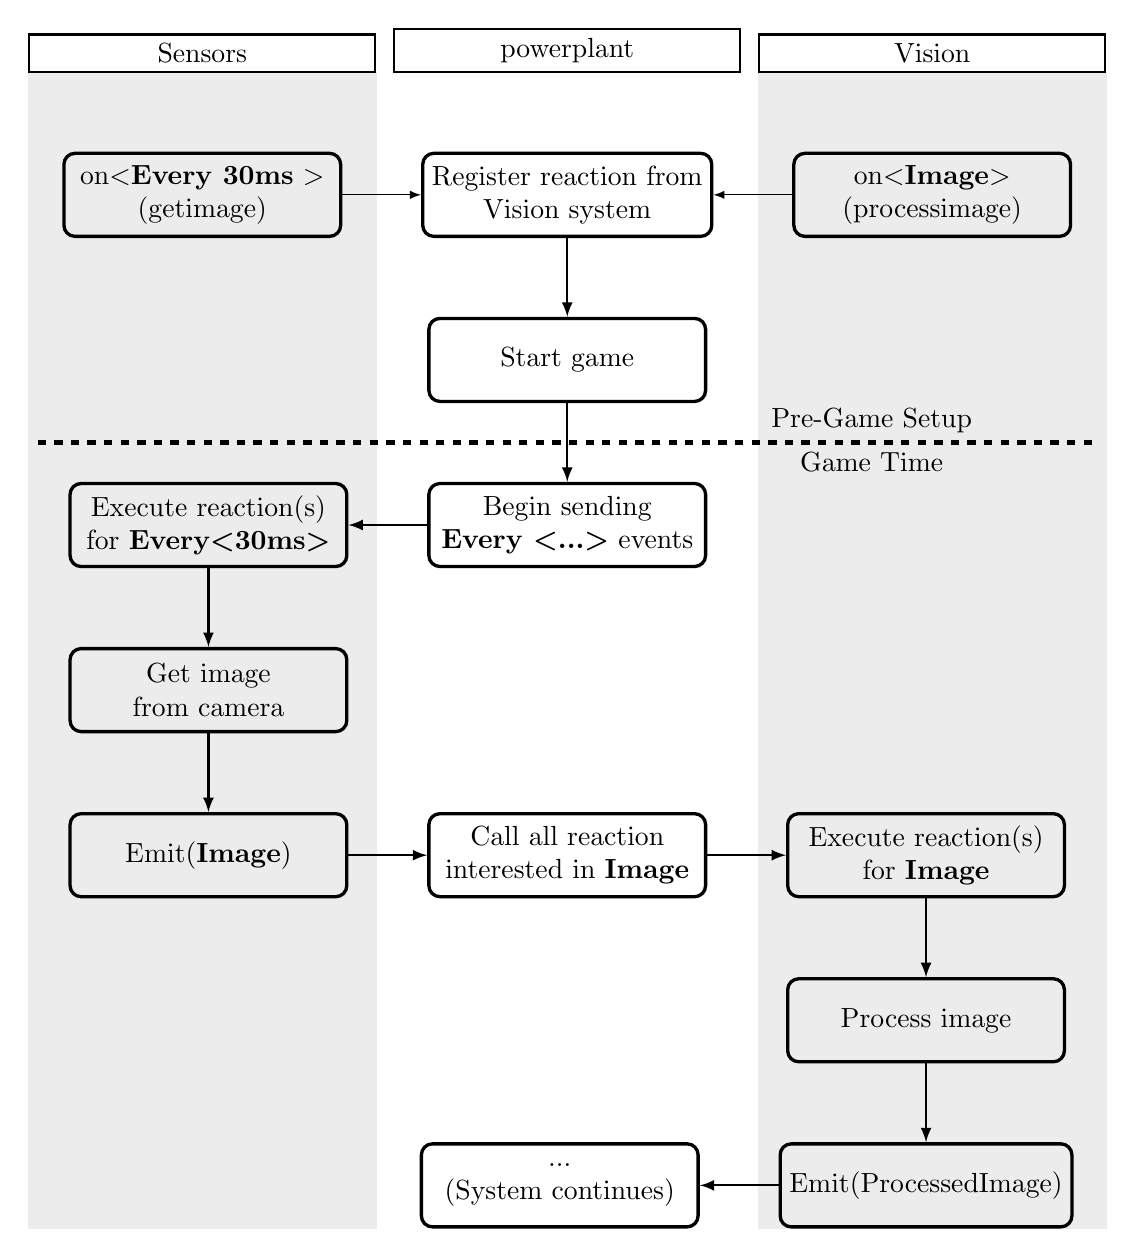
\begin{tikzpicture}[>=latex,
					block/.style={
						rectangle,
						rounded corners,
						draw=black, very thick,
						minimum height=3em,
						minimum width=10em,
						align=center
					},
					header/.style={
						rectangle,
						draw = black, thick,
						minimum height=1.2em,
						minimum width=12.5em,
						align=center
					},
					every join/.style={->, thick},
					chained/.style={every node/.style={on chain}}
				]
					\begin{scope}[start chain=going below, chained]

						% Draw the Register node and setup the following blocks to have arrows
						\node [block,join] (register) {Register \gls{reaction} from \\ Vision system};
						\begin{scope}[start branch=on going right, every join/.style={<-}]
							\node [block,join] (onimage) {on\textless \textbf{Image}\textgreater
							\\(processimage)};
						\end{scope}

						% Draw the on Every node
						\begin{scope}[start branch=on going left, every join/.style={<-}]
							\node [block,join] (onevery) {on\textless \textbf{Every 30ms}
							\textgreater\\(getimage)};
						\end{scope}

						% Start game node
						\node[block,join] (start) {Start game};

						% In Game every node
						\node [block, join] (runtimeStart) {Begin sending\\\textbf{Every
							\textless ...\textgreater} events};

						% Sensor Reactors node
						\node [block, join, on chain=going left] {Execute \gls{reaction}(s) \\for
							\textbf{Every\textless 30ms\textgreater}};

						% Get Camera Image Node
						\node [block, join] {Get image\\from camera};

						% Emit Node
						\node [block, join] {Emit(\textbf{Image})};

						% Image Call Node
						\node [block, join, on chain=going right] {Call all \glspl{reaction}\\interested
							in \textbf{Image}};

						% Execute Reactions Node
						\node [block, join, on chain=going right] {Execute \gls{reaction}(s)\\for
							\textbf{Image}};

						% Process Image Node
						\node [block, join] {Process image};

						% Emit Processed Image node
						\node [block, join] {Emit(ProcessedImage)};

						% Continuation Node
						\node [block, join, on chain=going left] (final) {...\\(System continues)};
					\end{scope}

					\coordinate (setuplineA) at ([xshift=-18em]$ (start) !.5! (runtimeStart) $);
					\coordinate (setuplineB) at ([xshift=18em]$ (start) !.5! (runtimeStart) $);
					\coordinate (setupTextPoint) at ([xshift=11em]$ (start) !.5! (runtimeStart) $);

					%% Setup dividing line and text
					\node [above] at (setupTextPoint) {Pre-Game Setup};
					\node [below] at (setupTextPoint) {Game Time};
					\draw [dashed, ultra thick, shorten >= -0.4cm, shorten <= -0.4cm]
						(setuplineA) -- (setuplineB);

					%% Add headers for the three threads
					\node [header,above=of onevery] (sensorsHeader) {Sensors};
					\node [header,above=of register] {\gls{powerplant}};
					\node [header,above=of onimage] (visionHeader) {Vision};

					%% Add the column backgrounds for Sensors and Vision
					\begin{scope}[on background layer]
						\filldraw [gray!15] (sensorsHeader.south west) rectangle
							(sensorsHeader.east |- final.south);
						\filldraw [gray!15] (visionHeader.south west) rectangle
							(visionHeader.east |- final.south);
					\end{scope}
				\end{tikzpicture}
				\caption {A flowchart example of how \textbf{On}, \textbf{Emit} and \textbf{Every}
					work}
				\label{fig:OnAndEmitExample}
			\end{figure}

			One of the key advantages of this design is that components are loosely coupled and only depend on the data format not changing.
			Therefore, you could replace the hardware dependent camera system with a new module that reads from a prerecorded video stream for testing purposes.
			It also means that adding a new component to the system merely requires that you know what sort of data you want to access.
			As there is a single way to get data, there is no longer a need to track down the obscure method used to access the needed data. Instead you simply tell the system the type that you require and the system locates it for you.

			Recent trends in computer hardware show that computational power increases are going to come from increasing the number of cores available to the system.
			Unfortunately the current system only takes advantage of at most two cores.
			The way that the system is currently architected enforces an artificial limitation on the resource utilisation of the system.
			It would be inefficient to attempt to type with most of your fingers removed.
			In a similar way not making use of all the resources on the platform limits the potential of the final result.
			The proposed architecture takes care of multithreading transparently so the \gls{nubots} team can
			focus on figuring out the important questions such ``can this robot fetch me a pizza?''.
			When a \gls{reaction} is triggered it doesn't necessarily run immediately.
			Instead the \gls{reaction} is put into a blocking priority queue and then executed on one of the many threads
			available to the \gls{powerplant} via a thread pool.
			For an example of how this system works see Figure~\ref{fig:PowerPlantThreadingOverviewDiagram} on page~\pageref{fig:PowerPlantThreadingOverviewDiagram}.

			% Power Plant Threading Diagram
			\begin{landscape}
			\begin{figure}[b]
				\centering
				\begin{tabular}{|l|l|l|l|}
					\hline
					Trigger                             & Task         & Emits            & Duration \\
					\hline
					\rowcolor{red!10}  Every 20ms       & Sensors      & SensorData       & 4ms \\
					\rowcolor{red!10}  SensorData       & Odometry     & OdometryData     & 3ms \\
					\rowcolor{red!10}  OdometryData     & Field Mapper & MapData          & 4ms \\
					\rowcolor{red!10}  MapData          & Map Combiner & Network\textless MapData\textgreater & 7ms \\
					\rowcolor{blue!10} Every 20ms       & Camera       & CameraImage      & 5ms \\
					\rowcolor{blue!10} CameraImage      & Vision       & ProcessedImage   & 7ms \\
					\rowcolor{blue!10} ProcessedImage   & Localisation & LocalizationData & 3ms \\
					\rowcolor{blue!10} LocalizationData & Behaviour    & MotorTask        & 2ms \\
					\rowcolor{blue!10} MotorTask        & Motors       & Nothing          & 2ms \\
					\hline
				\end{tabular}

				\vspace*{1 cm}

				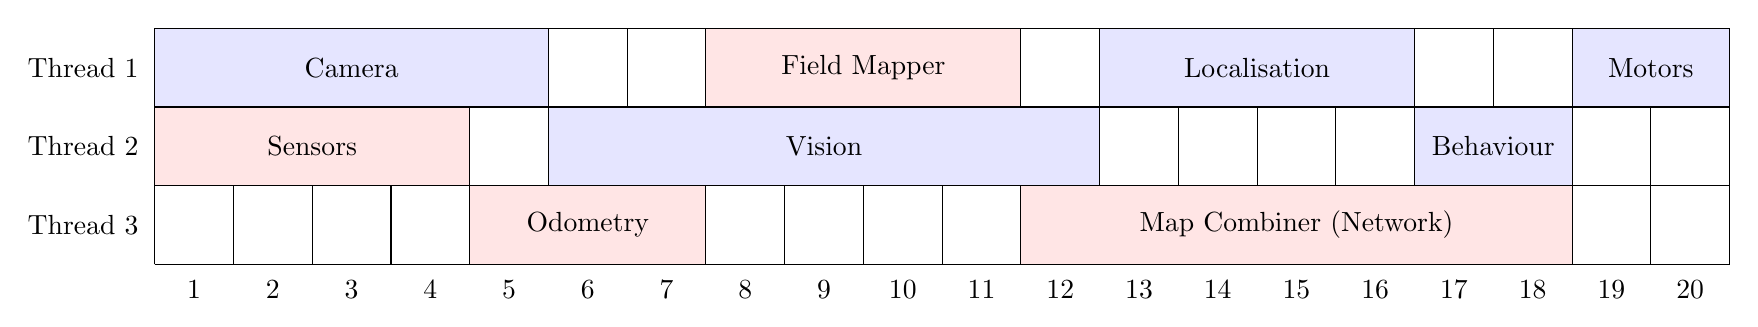
\begin{tikzpicture}

					\begin{scope}[
						task/.style={draw=black},
						cameratriggered/.style={fill=blue!10},
						sensortriggered/.style={fill=red!10}
					]

						\draw (1, 1) grid (21, 4);

						%% Thread 1
						\draw[cameratriggered, task] (1, 3) rectangle node {Camera} (6, 4);
						\draw[sensortriggered, task] (8, 3) rectangle node {Field Mapper} (12, 4);
						\draw[cameratriggered, task] (13, 3) rectangle node {Localisation} (17, 4);
						\draw[cameratriggered, task] (19, 3) rectangle node {Motors} (21, 4);

						%% Thread 2
						\draw[sensortriggered, task] (1, 2) rectangle node {Sensors} (5, 3);
						\draw[cameratriggered, task] (6, 2) rectangle node {Vision} (13, 3);
						\draw[cameratriggered, task] (17, 2) rectangle node {Behaviour} (19, 3);

						%% Thread 3
						\draw[sensortriggered, task] (5, 1) rectangle node {Odometry} (8, 2);
						\draw[sensortriggered, task] (12, 1) rectangle node {Map Combiner (Network)} (19, 2);

						% Row labels
						\node[anchor=east, inner sep=0] at (.8, 3.5) {Thread 1};
						\node[anchor=east, inner sep=0] at (.8, 2.5) {Thread 2};
						\node[anchor=east, inner sep=0] at (.8, 1.5) {Thread 3};

						% Column Labels
						\foreach \i in {1,...,20} {
							\node[anchor=north, inner sep=0] at (\i + .5, .8) {\i};
						}
					\end{scope}

				\end{tikzpicture}
				\caption {An overview of the \gls{powerplant} threading system}
				\label{fig:PowerPlantThreadingOverviewDiagram}
			\end{figure}
			\end{landscape}

			The client has also expressed how important it is that the robots be able to easily communicate.
			Networking is a difficult and error-prone process which is why it is imperative that the architecture provide a simple mechanism for robots to communicate.
			The proposed architecture allows you to treat \glspl{reactor} on other robots as potential targets for your data.
			This means you can emit data on one robot and receive it on any of the other robots.
			See Figure~\ref{fig:NetworkExampleDiagram} on page~\pageref{fig:NetworkExampleDiagram} for an example of how the networking system allows robots to cooperate and share data.

			% Networking diagram
			\begin{figure}[b]
				\centering
				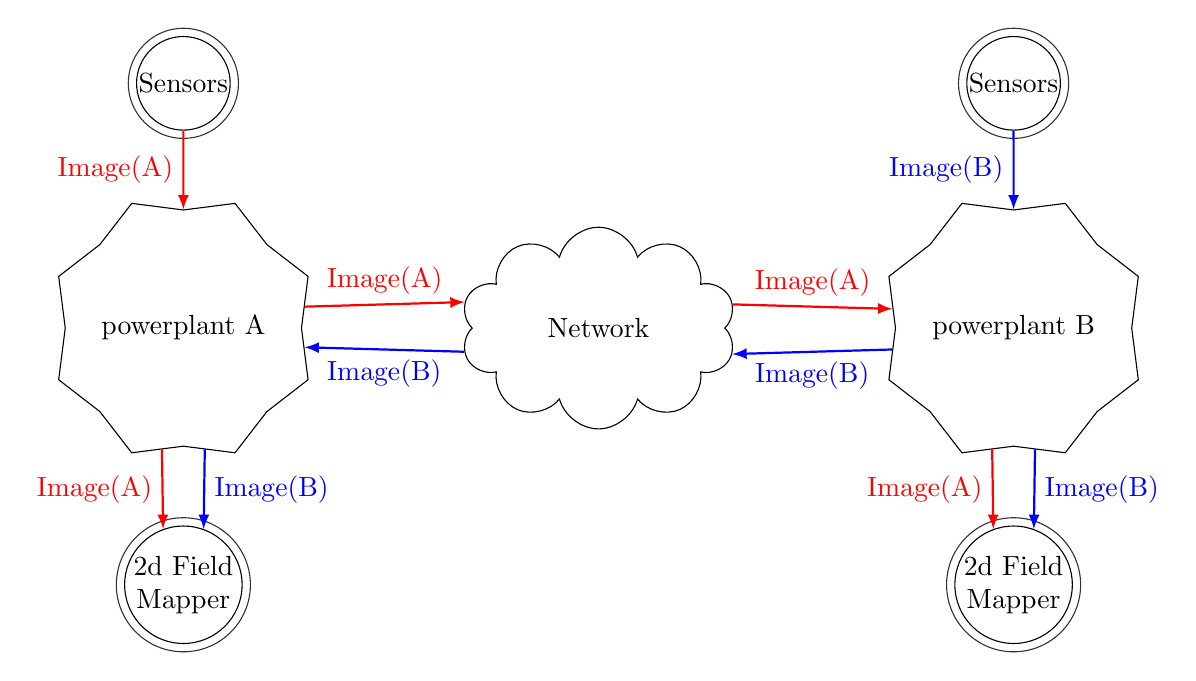
\begin{tikzpicture}[x=15em,y=5em,>=latex,
					A/.style={red},
					B/.style={blue}]

					%%% Left Power Plant
					\node at (0, 0)
						[draw,star,star points=8,star point ratio=0.875,minimum width=3cm]
						(plantA) {\gls{powerplant} A};
					\node [above=of plantA,reactor] (sensorsA) {Sensors};
					\node [below=of plantA,reactor,align=center] (fieldmapperA) {2d Field\\Mapper};
					\path [A, write] (sensorsA) edge node[A,left] {Image(A)} (plantA);
					\path [A, read] (fieldmapperA.110) edge node[left] {Image(A)} (plantA.260);
					\path [B, read] (fieldmapperA.70) edge node[right] {Image(B)} (plantA.280);

					%%% Right Power Plant
					\node at (2, 0)
						[draw,star,star points=8,star point ratio=0.875,minimum width=3cm]
						(plantB){\gls{powerplant} B};
					\node [above=of plantB,reactor] (sensorsB) {Sensors};
					\node [below=of plantB,reactor,align=center] (fieldmapperB) {2d Field\\Mapper};
					\path [B, write] (sensorsB) edge node[left] {Image(B)} (plantB);
					\path [A, read] (fieldmapperB.110) edge node[left] {Image(A)} (plantB.260);
					\path [B, read] (fieldmapperB.70) edge node[right] {Image(B)} (plantB.280);

					%%% Network & Network Connections
					\node at (1, 0) [draw,cloud,cloud puffs=10,minimum width=3.5cm]
					(network) {Network};

					%% Plant A connections
					\path [A, write] (plantA.10) edge node[A, above] {Image(A)} (network.169);
					\path [B, read] (plantA.-9) edge node[B, below] {Image(B)} (network.190);

					%% Plant B connections
					\path [A, read] (plantB.171) edge node[A, above] {Image(A)}  (network.10);
					\path [B, write] (plantB.190) edge node[B, below] {Image(B)} (network.-11);

				\end{tikzpicture}
				\caption {An example of how robots can communicate camera data over a network to
					build a 2d map of the field}
					\label{fig:NetworkExampleDiagram}
			\end{figure}

			\todo[inline] {Expand the description of the Proposed Architecture}
			\todo[inline]{Explain the diagram that all the components are loosely coupled}

	\section{Non-Goals}
		This section addresses areas of the system that are out-of-scope for the proposed architecture.
		The proposed architecture will make no effort to address these issues directly however some out-of-scope
		components will benifit indirectly from improved architectural consistency.
		
		\subsection{Algorithm Changes}
			The \gls{nubots} system contains a number of complicated mathematical systems that are used by the robot
			to analyse the world, make decisions and perform other useful functions. 
			The proposed architecture will not change these algorithms beyond any neccecary changes required to
			integrate them into the new architectural style.
			
			This means that while we might modify how the vision algorithm gets it's inputs we won't be modifying the
			mathematical algorithm used to classify objects.

		\subsection{Hardware Changes}
			As far as the proposed architecture is concerned it is targeting an abstract computing platform with no specific hardware
			available to be identified. 
			
			We assume that there is some form of networking and processing but beyond that we impose no requirements on the
			existing or future hardware. Furthermore, the proposed architecture will not recommend or require any changes to the robotic
			hardware in order to run.

	\section{Scenarios}
		This section covers some common scenarios in robotics programming and how they would be resolved 
		using both the existing and proposed architecture.

		\subsection{New Functionality Added to System}
			The robot currently consists of several integrated components allowing it to play soccer.
			However, to enhance its ability to play effectively, new components may be added to the system.
			These components will either augment existing abilities or provide new functionality.

			\paragraph{Scenario} Due to a recent rule changes in the 
			\emph{\gls{robocup} humanoid division}~\cite[Section 1.2]{humanoid2013rules}, the goal posts are no longer different colours.
			Therefore, a new component must be added to the robot's software allowing it to determine the
			direction it is facing. In the event that the robot falls over this component would break the
			field symmetry and reorient the robot. The component responsible for finding the direction would
			require access to existing sensor input and its output would need to influence the localisation
			system. The team has already developed a system that is able to determine the direction the
			robot is facing by looking at features above it. All that remains is to integrate this with the current codebase.

			\subsubsection{Current System}
				To solve this problem we need to modify vision such that it can classify
				new inputs from the camera for the compass system. 
				We also need to add a new Behavior to allow the robot to look up.
				
				Modifying vision also means we need to understand how sensors, vision and blackboard each interact
				to retrieve the camera data. 
				We then need to hook the compass component into the vision system which requires modifications to both vision
				and blackboard.
				Once the new compass component itegrated with vision we also need to integrate it with localisation. 
				This involves a deep understanding of how localisation interacts with the blackboard and job systems and
				requires us to modify localisation, blackboard and the compass component.
				
				We then need to add a new behavior to the system to allow the robot to look up.
				This is no simple feat and involves modifying the core code of the Job, Motion and Behavior components while also understanding
				how each of them interact with each other, the job queue and blackboard.
			\subsubsection{Proposed System}
				This problem still requires that we add a new behavior.
				However we only need to modify vision's internals to add the new classification mechanism.
				We don't need to modify sensors and both blackboard and jobs no longer exist.
				
				Modifying the vision \gls{reactor} merely requires you to understand the incoming data and the vision system itself.
				Additionally, modifying behavior no longer requires that you understand the job and blackboard systems. 
				Instead you simply modify the motion component directly to be able to handle the new type of movement.

				Integration with localisation is much easier, we simply use the standard \gls{powerplant} emit/on mechanism to send the data to localisation.
				
				All of the communication between components uses the consistent \gls{powerplant} interface. This means that if you
				understand how to communicate with \gls{powerplant} then you understand how to communicate with every other component
				in the system.

		\subsection{Networking with other Robots}
			Many modules within the robots code can benefit from information gathered by other robots on their team. Sharing information such as the position of objects on the field and each robots current action allows better co-ordination of the team. Another advantage provided by networking
			is the opportunity for distributed computing on computationally or spatially intensive problems.
			
			\paragraph{Scenario} The \emph{\gls{nubots}} team have decided to improve their behaviour system to promote better teamwork between the robots. To facilitate this, the robots need an easy method to communicate their intentions to each-other across the network. The networking
			system needs to serialise the data from the behaviour system and deserialize this data on the receiving robots.
			
			\subsubsection{Current System}
				The current system performs networking at the socket level. This means each component
				that wants to communicate over the network needs to interact directly with sockets in order
				to communicate information.
				
				To implement this behaviour sharing mechanism a new packet type needs to be declared and a deep
				understanding of Win32 sockets, POSIX sockets and the existing network code is needed. Once the new
				packet is defined serialisation methods need to be written to convert it to a network compatible representation
				and back. Custom network code then needs to be written for the behaviour system to handle sending/receiving the
				networked data to ensure it is used correctly.
				
				Once the network transfer is complete the behaviour system then needs to be modified to utilise the new information.
				\todo[inline]{Write how the current system would resolve or does resolve this scenario}
			\subsubsection{Proposed System}
				The proposed architecture provides networking as part of the standard \gls{powerplant} interface.
				The first step is to define a new packet which can be done with either raw C++ classes or 
				google protocol buffers. Once that packet is defined you also need to add a network event handler
				to the Behaviour class which is a tiny modification in the proposed architecture.
				
				Once the handler is hooked up you simply use the standard api tools to send the networked packet
				between the robots. The architecture will handle details like serialisation, sockets and other network
				issues.
				
				As with the existing architecture you still need to modify the behaviour system to utilise the new data.
				\todo[inline]{Write how the proposed system would resolve this scenario}

		\subsection{Moving to a new hardware platform}
			Currently there are many robotic platforms that are available for the development of autonomous
			robotic systems. In previous years the \emph{\gls{nubots}} team have made use of the \emph{Sony AIBO},
			the \emph{Aldebaran Nao} and the \emph{Robotis DARwIn-OP} platforms. Additional robotic platforms will be used as technology progresses, requiring that the code be ported to the new platform.
			Ideally this action will result in a minimal number of changes to the code base.

			\paragraph{scenario} After a number of years, the Darwin-OP platform has become obsolete and a new platform, the Super Turbotron 5000, has been selected as its replacement. It has twenty
			additional degrees of freedom, stereo vision and two giant laser cannons. The system must be
			adapted to be able to utilise these changes with a minimal amount of impact to the existing codebase, as well as being able to still operate on the Darwin-OP during the transition.

			\subsubsection{Current System}
				The current system handles platform changes through a long and complicated chain of conditional compilation. There are
				more then 10 different components that rely on compiler flags to determine what platform they are targeting. This is a 
				complex change that affects the majority of the system and requires someone who understands the entire system.
				
				New components would need to be written to replace all of the hardware dependant components. This includes reading sensors,
				moving motors, kinematics and anything else that talks to the robot hardware. Additionally all the systems that talk to the affected
				components will also need to be modified. Typically this cascades to a system-wide modification.
				\todo[inline]{Write how the current system would resolve this scenario}
			\subsubsection{Proposed System}
				Because of the loose coupling between components it's only necessary to replace the components that directly depend on
				robot hardware. All low-level conditional compilation is rendered obsolete in the proposed architecture with only a skeleton
				remaining to tell the system which high-level components to activate.
				
				The majority of the system would remain unchanged. New components for hardware would still need to be written and
				old components may need to be updated to take advantage of new hardware.
				\todo[inline]{Write how the proposed system would resolve this scenario}

		\subsection{Debugging bad Data}
			\begin{quote}``Debugging is twice as hard as writing the code in the first place. Therefore, if you write the code as cleverly as possible, you are, by definition, not smart enough to debug it.'' - Brian Kernighan\end{quote}
			One of the most useful techniques available for software debugging is being able to see inputs and outputs for a section of code. Once the data that enters a section
			of code is known, the remainder of the code can be analysed by hand to ensure that each
			step has the expected result. Tracing the data through the system to where the unexpected results start reveals the source of the problem.

			\paragraph{Scenario} The \gls{nubots} team have encountered a problem where the robot after
			receiving a notification that it kicked an own goal, will proceed to breakdance instead
			of hanging its head in shame. They have identified that this activity is due to the
			\em{Breakdance} action being performed instead of the expected \em{SadRobot} action. However, they are unable to identify why this action is being performed and need to trace the source
			of this logical error.

			\subsubsection{Current System}
				In the existing system tracing is done through manually adding print statements to the code in the 
				affected areas. Some systems have the ability to write their data to the network to be viewed in real
				time but this is provided on a per-component basis and the exact mechanism differs for each components.
				
				For this particular problem trace statements need to be added to the Behaviour, Motion and Job systems to determine
				why this particular job is called and why the robot is kicking it's own goal in the first place. After these statements are added
				the \gls{nubots} team then needs identify the issue through the trace logs, write a fix and then run it live on the robot. If the 
				fix fails it's back to step 1. Repeat until the bug is fixed.
				\todo[inline]{Write how the current system would resolve this scenario}
			\subsubsection{Proposed System}
				In addition to standard logging capabilities the proposed architecture also provides the ability to capture
				the entire input sequence for a particular component. This means you can capture the exact inputs that
				caused the robot to kick an own goal and then breakdance. Once you've captured those inputs you can then
				turn them into a unit test which in many cases can be run independently from the robot. 
				
				Once you've translated the input into a unit test you then need to write your fix. However you don't
				need to deploy your fix you can instead simply run the unit test and see if it passes. If the unit test passes
				you simply deploy to the robot and the problem is solved.
				
				This approach also has the benefit of slowly building up a library of unit and regression tests against known bugs.
				\todo[inline]{Write how the proposed system would resolve this scenario}

		\subsection{The Robot is used to perform a new task}
			Robotics is an ever expanding field of research with robots being applied to an
			increasing number of tasks. Each of these tasks are often performed on the same robotic
			platforms and need to perform similar tasks. This provides a huge opportunity for code
			reuse amongst these tasks. However, code that is difficult to understand, or separate
			from the surrounding code may be ignored in favour of rewriting the required
			functionality.

			The \gls{nubots} team have been asked to add dancing capabilities to the robot to help market the 
			university. The university wants the robot to be able to dance to a beat and compete in 
			``So you think you can RoboDance''. The \gls{nubots} team realises that some of their existing
			code can be leveraged to build the dance subsystem.

			\subsubsection{Current System}
				In the existing architecture reuse of code is primarily achieved by copy+paste. This is 
				especially evident in places where there are multiple implementations of the same concept.
				
				Allowing the robot to dance requires a new behaviour module that contains the dance state
				machine. Additionally the sensor system will need to be modified to provide sound information
				to the new dance component. 
				
				The kinematics model in the existing system is also very useful for dancing. Unfortunately access
				to the kinematics model is very difficult in the current system requiring a lot of hoop jumping to
				get access to the appropriate data. 
				\todo[inline] {Properly describe the issues with accessing kinematics}
				\todo[inline]{Write how the current system would resolve this scenario}
			\subsubsection{Proposed System}
				Create a new sound \gls{reactor} that emits sound events. 
				Create a new sound analysis \gls{reactor} that determines the beat and emits
				the "feel" of the song.
				Have behaviour react to the "feel" data and select an appropriate scripted dance move.
				Motion runs the dance.
				\todo[inline]{Write how the proposed system would resolve this scenario}





	\section{Requirements}
		
		\todo[inline]{add an introduction to non goals and remove the instructions}
		{
		\em % This is the instructions
		This is the nitty-gritty section of the document. You can expect this section to be many
		times longer than any other section. Here we need to list every single requirement: What it
		is, why it's important, how we can test if we've achieved it and any important details about
		the requirement.

		One of the most important things to include here are any decisions and assumptions that have
		been made. For example:
		}

		\subsection{Multiprocessing}
			\requirement{The architecture must take advantage of all CPU cores}

			The existing system is currently only able to take advantage of two cores, and one of
			those cores spends a lot of time doing very little work. Unfortunately writing
			multithreaded code is difficult and distracts programmers from more important things
			such as improving the speed at which a robot can backflip by 5\%. To account for this
			the proposed API must provide a way for programmers to easily utilise the full CPU power
			of any robot platform.

			This requirement is going to become increasingly important as time goes on. The current
			trend in computing performance is to add more cores and in the cutthroat world of
			robotic soccer it is of paramount importance that we utilise all of our resources.

			From an API point of view the ideal acceptance test for this requirement is to determine
			how often a programmer needs to think about multithreading at all. We could analyse the
			code to determine what sections need to include multithreaded primitives and from that
			percentage determine how many times the API failed to provide the proper multithreaded
			abstractions.

			From a performance and hardware point of view we can measure CPU utilisation on various
			platforms and compare it to the old system.

			Technical Note: We're assuming that we aren't going to be using many single-core
			machines. The API should still support single threaded machine but from a performance
			point of view we're assuming that additional cores is the way to go.

		\subsection{Robot Platforms}
			\requirement{The architecture must be portable to new platforms}

			The existing system has a lot of complicated logic that is used to support a few
			different platforms. It's currently not possible to easily swap out the Darwin motor
			components for an AIBO or Nao motor component due to the tight coupling of systems.

			The new architecture should provide a way to easily slot in platform dependant
			components. For example it should be possible to remove the hardware-dependant Darwin
			camera component and replace it with an AIBO component with minimal to no modification
			of other components.

			Portability can be measured by determining the amount of code that depends on specific
			hardware or platforms. For this exercise Unit Tests can be considered another platform
			so we could determine the portability by replacing hardware-dependant components with
			mock components.

			Technical Note: Obviously if the format of the data changes the systems that rely on
			that data need to change as well. We're looking to reduce unnecessary changes due to API
			bloat.

		\subsection{Performance}
			\requirement{The architecture must have acceptable performance}

			Robotic platforms have very strict requirements about how often motors need to be sent
			commands. If these performance requirements aren't met the robots are approximately as
			useful as a very ambitious block of wood. Because of these requirements the proposed
			architecture cannot impose large processing or resource costs to the existing system.

			A good example of a system that imposes heavy performance costs is ROS (Robot Operating
			System). ROS has made a number of trade-offs to facilitate distributed multi-language
			multi-platform systems but those trade-offs have resulted in unacceptable performance
			implications for smaller robots such as the Darwin.

			The proposed architecture should be optimised to run efficiently so it doesn't take
			valuable resources away from critical computations. Ideally the architecture should be
			structured in such a way that it can assist the \gls{nubots} team in writing efficient code.
			The first key indicator of performance is to determine the ratio of time used by the
			architecture vs. the time taken by actual components. Ideally the ratio should be so
			small as to be practically insignificant. A good architecture should also provide the
			tools to measure performance.

			We can also measure the speed of the old architecture vs. the new architecture to
			determine what improvements have been made.

		\subsection{Component Interfaces}
			\requirement{The architecture must promote consistent interfaces between components}

			In the existing system there are a number of ways components can communicate all of
			which have their own conventions, quirks and pitfalls. The biggest problem with this is
			it greatly increases the complexity of the system and also causes increased coupling due
			to all the different ways components can communicate.

			The proposed system needs to provide a unified mechanism for components to communicate.
			However this unified mechanism shouldn't force us to remove any existing functionality
			and as such must be able to accommodate or replace any of the existing communication
			styles. By providing a unified mechanism we can greatly reduce the complexity of the
			system.

			This requirement can be measured by analysing the mechanisms that components use to
			communicate. For example we can look at all the places the Camera system communicates
			with the Vision system and determine the number of unique ways in which they
			communicate. Additionally we can measure the suitability of the unified mechanism by
			ensuring that it doesn't force us to remove any existing functionality.

		\subsection{Adding Components}
			\requirement{The architecture must make it easy to add new components to the system}

			Adding a new component to the existing system is currently a highly perilous journey of
			discovery involving knowledge of huge portions of the existing system to achieve and
			copious amounts of prayer. Because the existing communication graph is basically a giant
			yarn ball held together by faith every new component exponentially adds more complexity
			to the existing system and makes the next new component even harder to add.

			This is one of the key components the new architecture needs to solve. Ideally if you
			want to add a new component you should only need to know about the inputs and outputs of
			your component. The proposed architecture must provide a mechanism to simplify adding
			new components to the system.

			This requirement is best measured by comparing it against the old system. Take some
			hypothetical component and look at how many systems you would need to touch to add it.
			For example we could consider adding a new behaviour system to handle catering at
			university functions. We could then analyse how many components would need to be
			understood and changed to add this new components we could also develop a metric for
			analysing the extent of the changes.

			\todo[inline]{Consider defining analysis metric in this document}

		\subsection{Networking}
			\requirement{The architecture must provide methods to easily perform network
			communication}

			Communication is a vital part of any team activity, without communication there is no
			way to work on team behaviour, or share useful information. The current system does have
			a networking solution. However it is difficult to use and this deters coders from using
			it to better the team abilities of the robots. By providing a simple and intuitive
			interface to send and receive networked data, a greater range of possibilities of team
			behaviour and distributed computing become accessible to the \gls{nubots} team.

			The new architecture must be able to automatically find and communicate with any robots
			that are currently on the network without configuration (auto discovery). It also must
			be able to serialise packets of data into a binary format for the majority of cases, and
			allow the user to provide a serializer for any edge cases. The cases that should be
			covered by the system as a minimum are any data type that contains only Plain Old Data
			(a container of basic data types only), or an instance of a
			Protocol Buffer~\cite{protobuf}.

			This requirement is measured by the amount of code that is required to both send and
			receive network packets from other robots, as well as how efficient the binary
			representation over the network is. For example, take the case of the two robots
			bragging about how they went after the game. Being robots, it would be inefficient to
			communicate using a natural language such as English they would not be able to convey
			their level of awesome quickly enough (running out of bandwidth), as such all
			information exchanged should be in a binary format. Also, as the robot is made up of
			many individual components, the communication between these components, must use the
			same communication channel, but have different origin and destination points

		\subsection{Debugging Tools}
			\requirement{The architecture must provide tools for debugging components}

			Debugging in the current system is a very difficult and painful process. Since all of
			the components are so tightly integrated with each other, this means that if an error
			occurs in one system, it is difficult to locate where the source of the error was. For
			example, in the current system an issue exists where if the camera is not connected, the
			vision system (the next system in the pipeline) will progress to the point of
			classifying the image before the robot crashes. This makes it appear that the bug is
			located in the vision system, however it is actually located in the camera reading
			system.

			The new architecture should provide tools within it that allow the debugging of both
			errors with the systems, as well as the performance between the systems. Using the tree
			style model of communication between components, it is possible to output this tree into
			a format that is understandable. This would allow the person debugging the system to see
			where each data packet that was used in the system of interest came from, and if enabled
			the contents of those data packets should also be available in order to replay the
			scenario that caused the error.

			These debugging tools can be measured by comparing the difficulty of tracing the source
			of data from one system to another.

			\todo[inline]{Expand this measurable for the debugging tools}

		\subsection{Testing}
			\requirement{The architecture must provide tools for unit testing individual components}

			Unit testing is a very important concept as it allows a number of tests to be performed
			on individual components in the system. This can help to identify and kill bugs before
			they even leave the development environment. By enforcing greater isolation between the
			components, the architecture is able to make it much easier to test an individual
			component by sending it fake data and validating the results.

			The system must provide a testing harness that makes it easy to test in isolation a
			component of the system. This testing harness should be able to wrap around any of the
			individual components that make up the system and, without modification to the component
			itself, send fake input to the component and capture and validate any output from that
			system. This should allow the system to be unit tested thoroughly such that the number
			of bugs that exist when the code is executed on the robot is much lower.

			This requirement is measured by comparing the difficulty of testing a component between
			the current system and the new system. This includes both the difficulty of extracting
			the component from the system to be tested without other components (isolating the
			component) as well as the difficulty of testing its API and results once it has been
			extracted from the system.

	\section{Extension Goals}
		This section will outline extra goals that are not requirements but would be useful to have
		if we have extra time. None of these should be implemented before a Requirement unless the
		requirement implementation trivially adds an extension.

		\subsection{The architecture could support ROS (Robot Operating System) integration}
			There are a number of components that could be useful from the existing ROS codebase.
			The proposed architecture could provide systems to make ROS component integration easy.
			Currently the existing system doesn't contain any facilities for ROS integration.

			Additionally no other \gls{robocup} teams have any degree of ROS support. Having ROS support
			would give us a crippling advantage over the other teams.

			This goal can be measured by checking if we can integrate a ROS component.

			\todo[inline]{Improve/extend. Validate the claim about other \gls{robocup} teams}

	\bibliographystyle{plain}
	\bibliography{references}
	
	\printglossaries
\end{document}
